\documentclass{article}
\usepackage[utf8]{inputenc}
\usepackage{mathtools, nccmath}
\usepackage{mathabx}
\usepackage{mathrsfs}
\usepackage{natbib}
\usepackage{graphicx}
\usepackage{cancel}
\usepackage{upquote}
\usepackage{pgfplots}
\usepackage{amssymb}
\pgfplotsset{width=10cm,compat=1.9}
\usepgfplotslibrary{external}
\tikzexternalize
\usepackage{hyperref}
\usepackage{xparse}
\usetikzlibrary{through}

\usepackage{tikz}
\usetikzlibrary{angles,quotes}

\newcommand{\handC}{\mathscr{C}}

\title{Mate 1: Curs \#0}
\author{Profesor: Radu Gologan}
\date{26 Septembrie 2019}

\DeclarePairedDelimiterX{\set}[1]{\{}{\}}{\setargs{#1}}
\NewDocumentCommand{\setargs}{>{\SplitArgument{1}{;}}m}
{\setargsaux#1}
\NewDocumentCommand{\setargsaux}{mm}
{\IfNoValueTF{#2}{#1} {#1\,\delimsize|\,\mathopen{}#2}}%{#1\:;\:#2}

\begin{document}
    
    \maketitle
        \subsection*{Obtinere Nota}
            Nota finala maxima este de 100 de puncte, iar pentru promovare este necesar un minim de 41 de puncte. Punctele se vor obtine dintr-un test final alcatuit din 5 probleme, care valoreaza 50 de puncte. Restul de 50 de puncte din nota finala se vor obtine din seminar. La seminar, 10 puncte vor fi acordate pentru prezenta, 10 vor fi acordate pe activitatea la seminar, iar restul de 30 de puncte vor fi obtinute din doua teste partiale, fiecare in valoare de 15 puncte, sustinute in saptamana a 8-a, respectiv saptamana a 13-a.
        \subsection*{Resurse}
            \href{https://www.facebook.com/groups/723259271431305}{Grup Facebook: CA-Mate1\_2019}\\
            \href{https://ro.scribd.com/doc/77477726/Tania-Luminita-Costache-Analiza-a-Culegere-de-Probleme}{Tania-Luminita Costache - Analiza a Culegere de Probleme}\\
            \href{https://www.youtube.com/channel/UCRcpjorgGE-3-Z-Sg5wu70Q}{Matematici pentru politehnisti - Canal de YouTube}\\
            \href{https://www.facebook.com/groups/846192945437641/}{Matematici pentru politehnisti - Grup de Facebook}\\
            \href{https://alexnegrescu.wordpress.com/}{Blogul personal al Dl. Prof. Negrescu}\\

    \clearpage

    \section{Aproximarea lungimii unui cerc cu ajutorul analizei matematice}
        Fie $\handC (O, 1)$, $A_1\ A_2\ A_3\ ...\ A_n$ un poligon regulat inscris in $\handC$ si $B_1\ B_2\ B_3\ ...\ B_n$ un poligon regulat circumscris lui $\handC$ a.i. segmentul $B_iB_{i+1}$ este tangent la $\handC$ in $A_i$ . Vom demonstra folosind principii de analiza matematica ca $P(\handC)=2\pi$.\\
        Vom demonstra ca perimetrele celor doua poligoane au acceeasi limita atunci cand $n \to \infty$.\\

        \def\myrad{3cm}% radius of the circle
        
        \begin{center}
            \begin{tikzpicture}
            
                \coordinate (O) at (0,0);
                \draw (O) node[circle,inner sep=1pt,fill] {} circle [radius=\myrad];
                \fill (O) circle[radius=2pt] node[below left] {O};
                
                \path (O) ++(60:\myrad) coordinate (A1);
                \path (O) ++(0:\myrad) coordinate (A2);
                \path (O) ++(120:\myrad) coordinate (An);
                \fill[black] (A1) circle[radius=2pt] ++(60:1em) node {$A_1$};
                \fill[black] (A2) circle[radius=2pt] ++(0:1em) node {$A_2$};
                \fill[black] (An) circle[radius=2pt] ++(120:1em) node {$A_n$};
                \draw (A1) -- (A2);
                \draw (An) -- (A1);
                
                \draw 
                  (0:\myrad) coordinate (deg0) -- node[midway,below] {1} (O) -- (60:\myrad) coordinate (deg60)
                  
                  pic [draw,angle radius=1cm,"$\frac{2\pi}{n}$" ] {angle = deg0--O--deg60};
                  
                \draw 
                  (60:\myrad) coordinate (deg60) -- node[midway,below] {} (O) -- (120:\myrad) coordinate (deg120)
                  
                  pic [draw,angle radius=1cm,"$\frac{2\pi}{n}$" ] {angle = deg60--O--deg120};
                  
                \draw [dashed, thick] 
                  (130:\myrad) coordinate (start)
                  (350:\myrad) coordinate (end)
                  pic [draw,angle radius=3.2cm] {angle = start--O--end};
            \end{tikzpicture}
        \end{center}
        Folosind teorema cosinusului:\\ $A_iA_{i+1} = \sqrt{2 - 2cos\left(\cfrac{2\pi}{n}\right)} = \sqrt{4sin^2\left(\cfrac{\pi}{n}\right)} = 2sin\left(\cfrac{\pi}{n}\right)$.\\
        Deci, perimetrul poligonului inscris in $\handC$ este $P_A(n)=2n\cdot sin\left(\cfrac{\pi}{n}\right)$.\\
        Din faptul ca $B_iB_{i+1}$ este tangent la $\handC$ in $A_i$, rezulta ca $\triangle OA_iB_i$ este dreptunghic in $A_i$\\ $\implies A_iB_i = tg\left(\cfrac{\pi}{n}\right) \implies B_iB_{i+1} = 2tg\left(\cfrac{\pi}{n}\right) \implies P_B(n) = 2n\cdot tg\left(\cfrac{\pi}{n}\right)$.\\
        Intrucat $P_A(n) < P(\handC) < P_B(n), \forall n \geq 3$, trecand la limita cand $n\to \infty$ vom avea:\\
        $$\lim_{n\to \infty}P_A(n) \leq P(\handC) \leq \lim_{n\to \infty}P_B(n) \iff$$
        $$\lim_{n\to \infty}2n\cdot sin\left(\cfrac{\pi}{n}\right) \leq P(\handC) \leq \lim_{n\to \infty}2n\cdot tg\left(\cfrac{\pi}{n}\right) \iff$$
        $$\lim_{n\to \infty}2\pi\cdot \cfrac{sin\left(\cfrac{\pi}{n}\right)}{\cfrac{\pi}{n}} \leq P(\handC) \leq \lim_{n\to \infty}2\pi\cdot \cfrac{tg\left(\cfrac{\pi}{n}\right)}{\cfrac{\pi}{n}} \iff$$
        $$2\pi \leq P(\handC) \leq 2\pi \iff P(\handC) = 2\pi\ \blacksquare$$
        
    \section{Aproximarea functiei $sin(x)$ pentru valori foarte mici ale lui $x$}
        $$\lim_{x\to0} \cfrac{sin(x)}{x} = 1 \implies\ x \lll,\ sin(x) \approx x $$
        $$\lim_{x\to0} \cfrac{x-sin(x)}{x^3} = \cfrac{1}{6} \implies\ x \lll,\ sin(x) \approx x-\cfrac{x^3}{6} $$
        \begin{center}
            \begin{tikzpicture}
              \draw[->] (-4,0) -- (4,0) node[right] {$x$};
              \draw[->] (0,-4) -- (0,4) node[above] {$y$};
              \draw[scale=1,domain=-3:3,smooth,variable=\x,black] plot ({\x},{sin(deg(\x))});
              \draw[scale=1,domain=-3:3,smooth,variable=\x,red] plot ({\x},{\x});
              \draw[scale=1,domain=-3:3,smooth,variable=\x,blue] plot ({\x},{\x-\x*\x*\x/6});
            \end{tikzpicture}
        \end{center}
        
        Se observa din graficul celor 3 functii $sin(x)$ - negru; $x$ - rosu si $x-\cfrac{x^3}{6}$ - albastru, ca cea de-a doua aproximare este mai precisa decat prima.\\
        
    \section{Aproximarea lui $\sqrt{2}$ folosind metoda tangentei}
        Fie $f : [0,\infty] \rightarrow \mathbb{R},\ f(x) = x^2-2$, sirul ${(x_n)}_{n\geq1},\ x_1 = 2,\ x_{n+1} = \cfrac{x_n^2+2}{2x_n}$ si punctele $P_i = (x_i,f(x_i)),\ \forall\ i \in \mathbb{N}^*$.\\ 
        Vom demonstra ca sirul ${(x_n)}_{n\geq1}$ este convergent, si are limita $\sqrt{2}$.\\
        \begin{center}
            \begin{tikzpicture}
            
                \def\mysqrt{1.414213}
            
                \draw[->] (-3,0) -- (3,0) node[right] {$x$};
                \draw[->] (0,-3) -- (0,3) node[above] {$y$};
                \draw[scale=.5,domain=0:2.8,smooth,variable=\x,black] plot ({\x},{\x*\x-2});
                \draw[->] (5,0) -- (11,0) node[right] {$x$};
                \draw[->] (8,-3) -- (8,3) node[above] {$y$};
                \draw[scale=.5,domain=0:2.8,smooth,variable=\x,black] plot ({\x+2*8},{\x*\x-2});
                \fill (0, -1) circle[radius=1.5pt] node[anchor=east] {$-2$};
                \fill (8, -1) circle[radius=1.5pt] node[anchor=east] {$-2$};
                \draw[scale=.5, dashed] (2,0) -- (2,2);
                \draw[scale=.5, dashed] (0,2) -- (2,2);
                \draw[scale=.5, dashed] (17.5,0) -- (17.5,0.25);
                \draw[scale=.5, dashed] (16,0.25) -- (17.5,0.25);
                \fill (1, 1) circle[radius=1.5pt] node[anchor=west] {$P_1$};
                \fill (8.75, 0.125) circle[radius=1.5pt] node[anchor=west] {$P_2$};
                \draw[shorten >=-1.5cm,shorten <=-1cm, color = red] (0.75,0) -- (1,1);
                \draw[shorten >=-1.5cm,shorten <=-1cm, color = red] (8.7083,0) -- (8.75,0.125);

            \end{tikzpicture}
        \end{center}
        Consideram tangenta la graficul functiei $f(x)$ in punctul $P_1$. Ecuatia tangentei este $y-f(x_1)={f^'}(x_1)\cdot(x-x_1) \implies x = \cfrac{x_1\cdot{f^'}(x_1)+y-f(x_1)}{{f^'}(x_1)}$ pentru $y=0 \implies x=\cfrac{2x_1^2 - x_1^2+2}{2x_1}=\cfrac{x_1^2 + 2}{2x_1}=x_2$, de unde rezulta ca $x_2$ este solutie pentru tangenta la $f(x)$ in punctul $P_1$. Prin inductie matematica, se poate demonstra recurenta sirului ${(x_n)}_{n\geq1}$.\\
        Folosind inegalitatea mediilor:\\
        \begin{equation}
            x_{n+1} = \cfrac{x_n^2+2}{2x_n} \geq \cfrac{2\sqrt{2x_n^2}}{2x_n}=\sqrt{2} \implies x_n \geq \sqrt{2},\ \forall\ n \geq 2
        \end{equation}
        \begin{center}
            $x_{n+1}-x_n = \cfrac{x_n^2+2}{2x_n} - x_n = \cfrac{2-x_n^2}{2x_n}$\\
        \end{center}
        \begin{equation}
            (1) \implies x_{n+1}-x_n \leq \cfrac{2-\sqrt{2}^2}{2\sqrt{2}} = 0 \implies x_n \searrow
        \end{equation}
        Ca urmare a teoremei lui Weierstrass:\\ $$(1),(2) \implies \exists\ l \geq \sqrt{2},\ a.i.\ \lim_{n\to\infty} x_n = l$$\\
        $$\lim_{n\to\infty}x_{n+1} = \lim_{n\to\infty} \cfrac{x_n^2+2}{2x_n} \iff l = \cfrac{l^2+2}{2l} \iff l=\sqrt{2}\ \blacksquare$$\\
        In continuare, vom studia viteza de convergenta a sirului $x_n$.\\
        Notam $y_{n+1} = x_{n+1}-\sqrt{2} = \cfrac{2+x_n^2}{2x_n}-\sqrt{2} = \cfrac{2 -2\sqrt{2}x_n+x_n^2}{2x_n}=\cfrac{{(x_n-\sqrt{2})}^2}{2x_n} = \cfrac{y_n^2}{2x_n}$.\\
        $x_n \geq \sqrt{2} > 1 \implies y_{n+1} < \cfrac{y_n^2}{2}$.\\
        $y_{n+1} < \cfrac{y_n^2}{2} < \cfrac{1}{2}\cdot{(\cfrac{y_{n-1}^2}{2})}^2 = \cfrac{y_{n-1}^4}{2^3}$.\\
        Se demonstreaza prin inductie matematica inegalitatea:\\
        $y_{n+1}<\cfrac{1}{2^{1+2^2+...+2^{n-1}}}\cdot y_1^{2^n} = \cfrac{y_1^{2^n}}{2^{2^n-1}}$.\\
        $y_1 = 2-\sqrt{2} > \cfrac{1}{2} \implies y_{n+1} < \cfrac{\left(\cfrac{1}{2}\right)^{2^n}}{2^{2^n-1}} = \cfrac{2}{2^{2^{n+1}}}$.\\
        Astfel, pentru a obtine o aproximare a lui $\sqrt{2}$ cu $k$ zecimale exacte:\\ $\exists\ n \geq\ 2\ a.i.\ y_n < \cfrac{2}{2^{2^n}} < 10^{-k} \implies 2^{2^n} \approx k\cdot\log_2{10} \implies n \approx log_2(log_2(k))$.\\
    \section{Calculul dimensiunii unei figuri}
        Consideram un segment de lungime 1, si un segment de lungime $\epsilon > 0,\ \epsilon \lll$
        \begin{center}
            \begin{tikzpicture}
            
                \draw [color=black,|-|] (0,0) -- (10,0) node[anchor=west]{$1$};
                \draw [color=black,|-|] (0,1) -- (0.5,1) node[anchor=west]{$\epsilon$};
            \end{tikzpicture}
        \end{center}
        Fie $n$ numarul de segmente $\epsilon$ necesare pentru a acoperi intregul segment.\\
        $(n-1)\cdot\epsilon<1<n\cdot\epsilon \implies n \approx \epsilon^{-1}$.\\ \\
        Consideram un patrat cu latura de lungime 1, si un patrat cu latura de lungime $\epsilon > 0,\ \epsilon \lll$
        \begin{center}
            \begin{tikzpicture}
            
                \draw [color=black] (0,0) -- (5,0) -- (5,5) -- (0,5) -- cycle;
                \draw [name=small,color=black] (0,0) -- (0,.5) -- (.5,.5) -- (.5,0) --cycle;
                \draw (2.5,2.5) node {$1$};
                \draw (.25,.25) node {$\epsilon^2$};
            \end{tikzpicture}
        \end{center}
        Fie $n$ numarul de patrate $\epsilon$ necesare pentru a acoperi intregul patrat.\\
        $(n-1)\cdot\epsilon^2<1<n\cdot\epsilon^2 \implies n \approx \epsilon^{-2}$.\\ \\
        Consideram un cub cu latura de lungime 1, si un cub cu latura de lungime $\epsilon > 0,\ \epsilon \lll$
        \begin{center}
            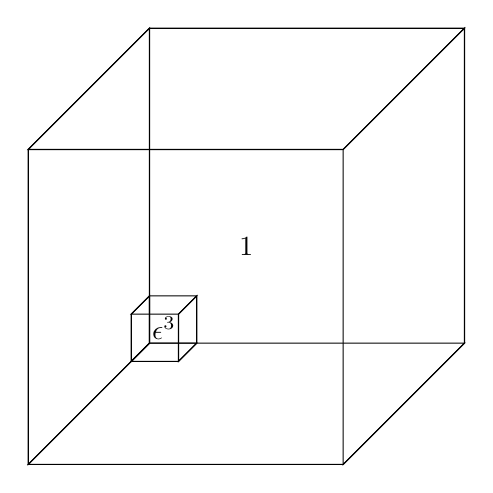
\begin{tikzpicture}
            
                \draw [color=black] (0,0,0) -- (0,0,4) -- (0,4,4) -- (0,4,0) -- cycle;
                \draw [color=black] (4,0,0) -- (4,0,4) -- (4,4,4) -- (4,4,0) -- cycle;
                \draw[color=black] (0,0,0) -- (4,0,0) -- (4,0,4) -- (0,0,4) -- cycle;
                \draw[color=black] (0,4,0) -- (4,4,0) -- (4,4,4) -- (0,4,4) -- cycle;
                \draw [color=black] (0,0,0) -- (0,0,.6) -- (0,.6,.6) -- (0,.6,0) -- cycle;
                \draw [color=black] (.6,0,0) -- (.6,0,.6) -- (.6,.6,.6) -- (.6,.6,0) -- cycle;
                \draw[color=black] (0,0,0) -- (.6,0,0) -- (.6,0,.6) -- (0,0,.6) -- cycle;
                \draw[color=black] (0,.6,0) -- (.6,.6,0) -- (.6,.6,.6) -- (0,.6,.6) -- cycle;
                
                \draw (2,2,2) node {$1$};
                \draw (.3,.3,.3) node {$\epsilon^3$};
            \end{tikzpicture}
        \end{center}
        Fie $n$ numarul de cuburi $\epsilon$ necesare pentru a acoperi intregul cub.\\
        $(n-1)\cdot\epsilon^3<1<n\cdot\epsilon^3 \implies n \approx \epsilon^{-3}$.\\ \\
        Notam $A \subseteq \mathbb{R}^2$ suprafata unei figuri, dimensiunea lui $A$ cu $d = dim(A),\ d \leq 2$ si $N(\epsilon) =\ numarul\ de\ patrate\ de\ latura\ \epsilon\ \lll\ necesare\ pentru\ a\ acoperi\ A$.\\
        In mod general, definim $d$ atunci cand $N(\epsilon) \approx \epsilon^{-d} \iff d \approx \cfrac{ln(N(\epsilon))}{ln\left(\cfrac{1}{\epsilon}\right)}$.\\
        
        Pentru $\epsilon=\cfrac{1}{2^n} \implies d = \displaystyle{\lim_{n\to\infty} \cfrac{ln\left(N\left(\cfrac{1}{2^n}\right)\right)}{ln(2^n)}}$.\\
        Intrucat $\exists\ d = \displaystyle{\lim_{n\to\infty} \cfrac{ln\left(N\left(\cfrac{1}{2^n}\right)\right)}{ln(2^n)}}$, $\displaystyle{\lim_{n\to\infty}ln(2^n)}=\infty$ si $ln(2^{n+1})-ln(2^n)=ln(2) \implies ln(2^n) \nearrow$, putem aplica lema Stolz-Cesaro:\\
        $d=\displaystyle{\lim_{n\to\infty}\cfrac{1}{ln(2)}\cdot ln\left(\cfrac{N\left(\cfrac{1}{2^{n+1}}\right)}{N\left(\cfrac{1}{2^n}\right)}\right)}$
    
        Pentru o mai buna intelegere, vizionati \href{https://www.youtube.com/watch?v=gB9n2gHsHN4}{Fractals are typically not self-similar} ce ofera o interpretare geometrica asupra problemei.
        
\end{document}